\documentclass[Main]{subfiles}
\begin{document}

\chapter{GUI}
\label{cha:gui}

The GUI was created using Matlab GUIDE. The GUI utilizes the encoder function described in section \ref{sec:EncImpl} and the decoder described in sections \ref{sec:decImplOv} through \ref{sec:decoderImpl}. The implementation details of the GUI are not in the scope of this report, but the source code is attached as appendix \ref{App:SourceCode}.
The GUI is shown in figure \ref{fig:meggittGUI}.

\begin{figure}[h]
    \centering
    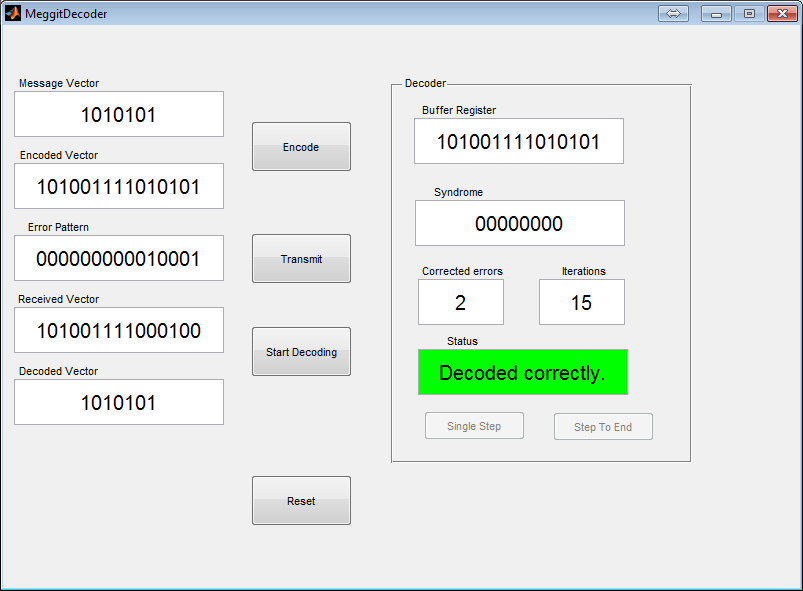
\includegraphics[width=0.65\textwidth]{figures/gui}
    \caption{Meggitt decoder GUI}
    \label{fig:meggittGUI}
\end{figure}

The following is a brief description of the elements of the GUI. Input to the encoding and decoding process is given using the input textboxes \emph{Message Vector} and \emph{Error Pattern}. The \textit{Encode} button invokes the encoder to create the \emph{Encoded Vector}. The \emph{Transmit} button applies the \emph{Error Pattern} to create the \emph{Received Vector}. The \emph{Start Decoding} button initializes the \emph{Buffer Register} of the decoder with the \emph{Recieved Vector}, and calculates the initial \emph{Syndrome}. Decoding can be done in \emph{Single Steps}, one iteration at a time. The button \emph{Step to end} will perform all remaining decoding iterations. The \emph{buffer}, \emph{syndrome}, \emph{corrected error} and \emph{iteration} counter will be updated after each decoding iteration to reflect the state of the decoder. When the decoding is complete, the status field will report the decoding status. Status is determined by checking if zero syndrome register and the buffer register matches the encoded vector.


\end{document} 